\documentclass[twocolumn]{article}
\usepackage{graphicx} % Required to insert images
\usepackage{listings} % Required for insertion of code
\usepackage{courier} % Required for the courier font
\usepackage{amsmath}
\usepackage{enumitem}
\usepackage{subfigure}
\usepackage{float}
\usepackage{url}
\usepackage{authblk}
\usepackage{wrapfig}
\usepackage[runin]{abstract}

\setlength{\absleftindent}{60pt}
\setlength{\absrightindent}{60pt}
\renewcommand{\abstractname}{}
\renewcommand{\absnamepos}{empty}

\begin{document}

%
% Title
%
\title{BrainActivity3D: Tool for EEG Signal Source Visualization}
\author{Anna Leontyeva, Dmytro Fishman and Ilya Kuzovkin} 
\affil{University of Tartu, Institute of Computer Science}

%
% Abstract
%
\twocolumn[
	\begin{@twocolumnfalse}
		\maketitle
		\begin{abstract}
		BrainActivity3D is a graphical application that localizes source of electroencephalographic (EEG) signal and renders it inside the 3D model of the human brain.  We apply independent component analysis (ICA) to estimate each electrode contributions and use source localization technique to pinpoint its location.
		\end{abstract}
		\section*{Bird's eye view}
	\end{@twocolumnfalse}
]

%
% Bird’s eye view
% note that section caption is defines few lines above
%

There are tiny cells, called \emph{neurons}, in our brain. Those cells communicate by exchanging electrical signal between each other. In some areas of the brain those cells align in a certain way, making it possible for otherwise weak electrical currents to penetrate through the scull, skin and other tissues and cause different areas of your head to have different electrical potential. 

This gives the ground for a neuroimaging technique called \emph{electroencephalography} (EEG). Sensitive electrical sensors, called \emph{electrodes}, are placed on the surface of the head, so that they can detect changes in the electrical potential, which, in their turn, imply that pattern of neuronal activity in your brain has changed.
We have in our possession one such portable EEG device:
\begin{figure}[H]
    \centering
    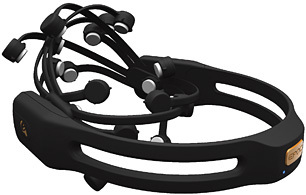
\includegraphics[width=0.56\linewidth]{../Images/emotiv.jpg} 
    \caption{Emotiv EPOC\textsuperscript{\textregistered}}
    \label{fig:emotiv_epoc}
\end{figure}
By analyzing its signal we can reconstruct the presumable location of the signal's source inside your head and overlay its position over the 3D model of a human brain. Visualizing this information in real time gives us the ability to observe which areas of your brain are active at the moment and associate this activity with different kinds of mental tasks.
\begin{figure}[H]
   \centering
   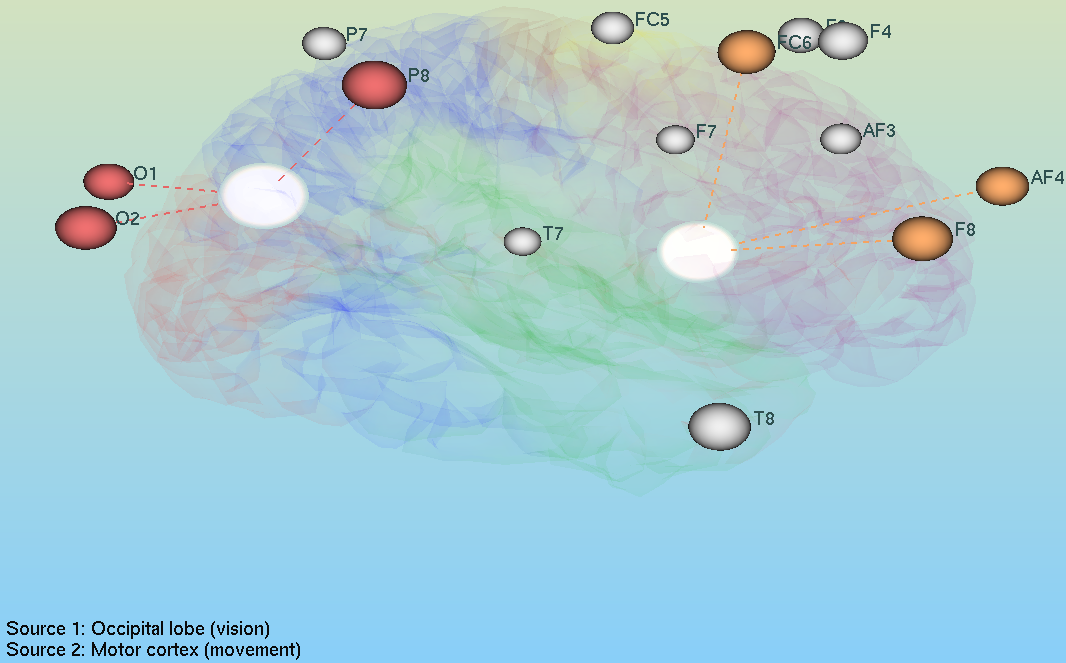
\includegraphics[width=1\linewidth]{../Images/screenshot.png} 
   \caption{Model of a human brain\cite{brainder}. Electrode locations are marked with spheres. Glowing blobs are estimated sources of the signal. List of sources, the lobe they appeared in and set of corresponding mental tasks are listed in the left lower corner.}
   \label{fig:screenshow}
\end{figure}

\thispagestyle{empty}
\clearpage

%
% Funcionality
%
\section*{Functionality}
The brain model can be displayed in two modes: solid mode and transparency mode (press "\texttt{T}" key or use contextual menu accessible by right mouse click to switch between the modes). Gray electrodes with corresponding labels indicate approximate position of the electrodes the Emotiv EPOC has. As soon as the signal will reach the system and first analysis results will be produced, some of the gray electrodes will be coloured according to the source they are influenced by. Estimated source position is indicated by an illuminated sphere inside the brain. The lower corner provides constant information about the number of sources, the lobes, where they appear and the activity these lobes correspond to. You can use mouse or the keyboard to rotate the brain. Use mouse scroll to zoom in and out. In case frames are changing to fast you can freeze the visualization by pressing "\texttt{P}" key.

%
% Technical details
%
\section*{Technical details}

\subsection*{The device}

Emotiv EPOC has 14 electrodes that measure electrical activity at 14 points on the surface of a human scull. The figure \ref{fig:epoc_placement} illustrates the position of the electrodes in 2D. The device has a sampling rate of 128 Hz and is able to pick up frequencies in the range from 0.1 to 50 Hz. The resulting data serves as an input for the BrainActivity3D application. It can be used both in real time by or reading pre-recorded data from file.
\begin{figure}[!h]
\begin{center}
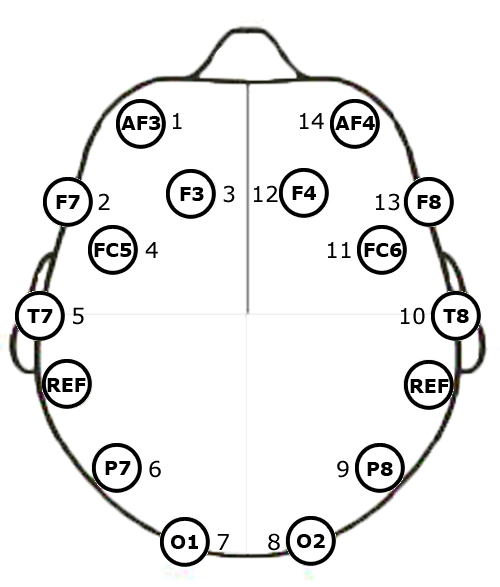
\includegraphics[width=0.5\columnwidth]{../Images/epoc_placement} 
\caption{Emotiv EPOC electrodes according to 10-20 system}
\label{fig:epoc_placement}
\end{center}
\end{figure}

\subsection*{Source localization}
The main purpose of the application is to find and visualize the position of the sources of the signal inside the brain. It is not as straightforward as it seems: source localization is considered to be ill-defined. In order to provide an algorithm for this task we need to make multiple assumptions. Firstly, we assume that source sends the electromagnetic wave to all 14 electrodes, thus, the strongest signal corresponds to the closest electrode. Secondly, the medium the signal travels through is assumed to be uniform. Thirdly we estimate fixed number of sources, which, biologically might not be a relevant model for the brain activity at all.

We approach the problem of source localization using one of the method proposed by Zukov et al. \cite{zhukov2000}. To estimate number of sources we perform Principal Component Analysis (PCA) and pick the number of components that describe more than $10\%$ of the variance of the data. After that we perform Independent Component Analysis (ICA) to find the contributions of each source to each electrode. The contributions are then used to allocate the signal using penalized least-square optimization.

\subsection*{Implementation}
We use \texttt{Python2.7} and \texttt{PyOpenGL} binding as the main tools for creating this application. \texttt{Emokit} library is used to communicate with the device. Implementations of PCA, ICA and least-square optimization are taken from packages \texttt{scikit-learn}\cite{scikit-learn} and \texttt{scipy}\cite{scipy}. Product is licensed under GNU General Public Licence version 3. You can find full list of dependecies and the source code of the project here: \url{https://github.com/kuz/BrainActivity3D}

%
% Installation
%
\section*{Installation and instructions}
Please use pre-built binaries for your system to run the application. If you would like to explore or change the application, please follow the instructions provided in the \texttt{README.md} file in the root catalogue of the project's source.

After you have successfully ran the application you can test it as follows:
\begin{enumerate}
	\item 	Position the device on a head of the subject according to the instructions provided with the device.
	\item Turn on the application and wait until source locations begin to appear
	\item Ask test subject to perform some muscular activity like:
		\begin{itemize}
			\item blink left or right eye
			\item clench teeth
			\item look at rapidly changing sequence of images
			\item perform motor activity
			\item engage in some type of mental task
		\end{itemize}
	\item Analyze the source positions change during the time and compare it to stimuli test subject provides. For examples if subject blinks with right eye, we expect the source to be on the right side in the frontal lobe near the electrode \texttt{F4}.
\end{enumerate}


%
% Conclusion
%
\section*{Conclusions and future work}
The initial goal of estimating the position of the source of the signal procuded during the mental task was not achieved: we were not able to confirm any correspondence between the mental task test subject was performing and the estimated location of the source. However the secondary objective was achieved partially: two test subjects claim that facial muscle activity was picked up correctly by the system and the estimated source location moved together with altering the source of muscular activity. Our future work could include such steps as:
\begin{itemize}
	\item Implementing support for more sophisticated and accurate EEG machine
	\item Properly exploring the problem of source localization and beamforming
	\item Do signal pre-processing and artefact removal
\end{itemize}
%
% Bibliography
%
\bibliographystyle{plain}
\bibliography{project_references}
 

\end{document}
